%!TEX root = ../main.tex

\graphicspath{{./figures/chapter1/}}

\chapter{FISH-quant}
\label{ch:chapter1}

\minitoc
\newpage

In this chapter I present FISH-quant v2, a computational framework for the analysis of \ac{smFISH} images.
FISH-quant v2 contains methods for every step of a \ac{FISH}-based study.
Based on a previous MATLAB package~\cite{mueller_fish-quant_2013}, I developed an improved and extended version, that is both scalable and modular and thus fulfills the requirement of a modern software tool.
The chapter mainly describes the work presented in the paper~\cite{Imbert_fq_2022} :

\begin{center}
	\color{green}
	A. Imbert, W. Ouyang et al. (2022), \textit{FISH-quant v2: a scalable and modular tool for smFISH image analysis}, RNA, pp. $\operatorname{786--795}$, iSSN: $\operatorname{1355--8382, 1469--9001}$.
\end{center}

\section{A Computational Framework for smFISH analysis}
\label{sec:framework}

In this section, I present the functionalities expected from a modern and efficient computational analysis framework for \ac{smFISH} images. 
%and review existing solutions.

\subsection{Detection, segmentation and pattern recognition}
\label{subsec:pipeline_stages}

% FISH in screening mode 
\ac{smFISH} permits the visualization of single \ac{RNA}s in cells and tissues and thus allows the exploration of the subcellular spatial distribution of \ac{RNA} molecules.
The analysis of \ac{smFISH} images aims at localizing and counting individual \ac{RNA}s in single cells and analyze their spatial configuration with respect to subcellular landmarks (e.g.~nuclear and cytoplasmic membranes).
It typically encompasses a sequence of interconnected steps, as illustrated in Figure~\ref{fig:pipeline}:
\begin{itemize}
	\setlength\itemsep{0.1em}
	\item detecting isolated and clustered \ac{RNA} molecules
	\item segmenting cells and the relevant cellular compartments such as nuclear and cytoplasmic membranes, mitochondria, centrosomes, etc. (depending on the focus of the study and the markers used)
	\item performing cell-level analysis of expression levels and \ac{RNA} localization patterns
\end{itemize}
%In multiplex smFISH studies, which are not subject of this PhD thesis, these steps are usually complemented by jointly analyzing different smFISH signals, i.e. point clouds of different types.

With recent technological advances, \ac{FISH} can be scaled up and therefore be applied in screening projects, where hundreds or thousands of experiments can be performed using a high degree of automation~\cite{safieddine_ht_smfish_2022}.
This then results in large and complex image datasets.

While such large-scale imaging methods can provide experimental data to understand \ac{RNA} localization at a systems level, they come at a price: the need for fully automated, robust image analysis and user-friendly software tools to analyze such data sets and to fully exploit their potential.
Several specifications can be defined a priori for such an analysis tool.
It should be simple enough to be mastered by non-experts, especially noncoders.
Yet, it should be flexible enough to address different experimental designs and rely on a common algorithmic backbone.
With the same modules, users should be able to both perform a high content screening analysis on a remote cluster, and a local analysis of a single image.
Finally, the software should integrate the latest generation of computer vision algorithms, in particular deep-learning-based methods for image segmentation.

\begin{figure}[]
    \centering
    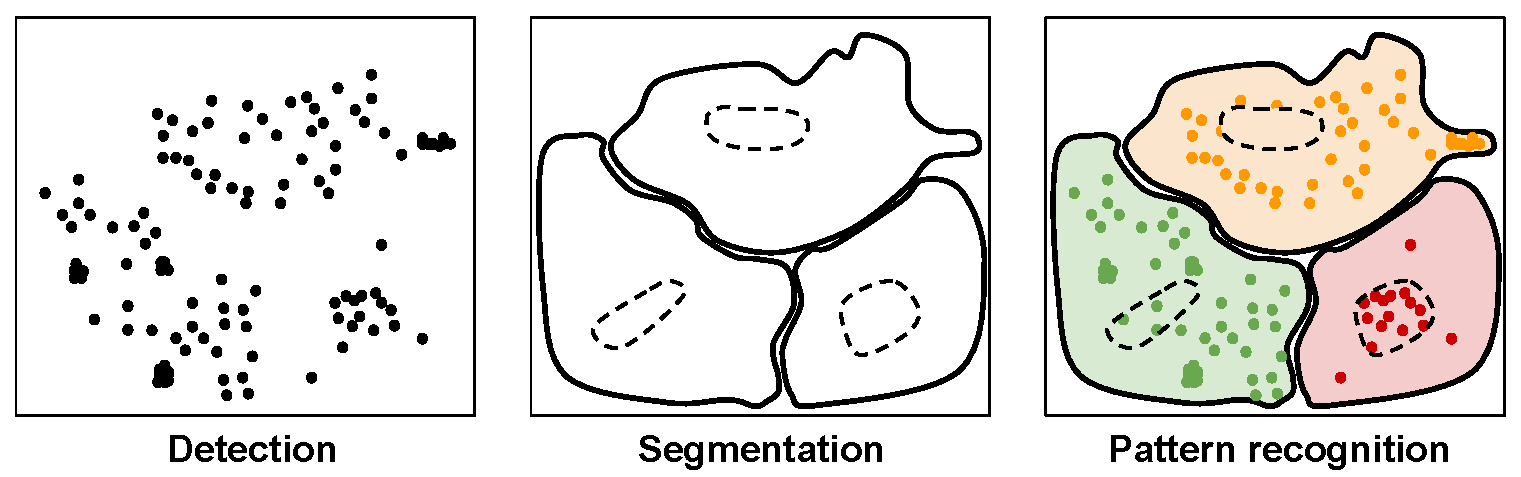
\includegraphics[width=\textwidth]{figures/chapter1/schema_pipeline}
    \caption[Computational pipeline for a smFISH study]{Computational pipeline I use as reference for a smFISH study}
    \label{fig:pipeline}
\end{figure}

\subsection{Related work}
\label{subsec:related_work_fishquant}

Processing a large-scale \ac{smFISH} study requires both specific methods to analyze \ac{RNA} distribution and more general techniques to read and manipulate images based on robust computer vision algorithms.
A \ac{FISH} analysis pipeline hence has to include several inter-dependent subtasks: an accurate \ac{RNA} detection method, the segmentation of relevant subcellular regions such as the cytoplasm and the nucleus, and preprocessing techniques to prepare the images (such that filtering, denoising or projection algorithms).
The obtained results can then be exploited to compute gene expression levels, by counting \ac{RNA} molecules, or develop localization features, to study non-random \ac{RNA} localization.

Specialized solutions for many of these subtasks exist, like BlobFinder~\cite{ALLALOU200958} for spot detection, but using them requires the end-user to assemble a complex analysis workflow, often across different programming languages.
This can be a daunting task, especially for wet-lab biologists with no formal training in computer science.

As an alternative, the development of complete analysis workflows can provide a modular and extensible pipeline for the analysis of \ac{RNA} abundance and localization.
As an example, the Pelkmans Lab published several papers illustrating the need for such complete and robust pipelines.
In~\cite{battich_image-based_2013, stoeger_computer_2015}, the authors develop a modular analysis pipeline permitting to analyze subcellular \ac{RNA} localization from their high-content screen.
The latter paper is a detailed protocol, that permits new users to perform their analysis quickly by providing a detailed description of the implemented approaches.
Further, the advantage of their modular approach, is that additional analysis tasks can be integrated to study related biological questions.
In latter work~\cite{battich_control_2015}, they reused parts of this pipeline to infer \ac{RNA} abundance per cell, and completed this analysis with morphological and phenotypic analysis to explain the observed heterogeneity in \ac{RNA} abundance.

These examples can provide several guidelines for future developments.
First, it is preferable to have a modular framework addressing every step in the \ac{smFISH} analysis pipeline, to facilitate usage.
Second, there is a balance to find between the scope of a framework, its flexibility, its scalability and the amount of user input required.
Lastly, to increase usability of a flexible framework, the analysis steps should be kept modular and be clearly explained.

While several tools exist for each stage illustrated in Figure~\ref{fig:pipeline}, there was - to our knowledge - no tool available that permits performing the entire analysis in one framework.
A complete analysis pipeline has then to be built by mixing these tools and requires some in-house developments, which can be daunting for non-specialists and may provide solutions that are unstable and difficult to scale.
For the segmentation, deep learning has become the method of choice with dramatic improvements in segmentation accuracy as compared to traditional methods.
Spot detection can be performed with different Python or Matlab packages.
However, assigning spot counts to segmentation results and the subsequent analysis of \ac{RNA} levels and RNA localization require custom-written code~\cite{stoeger_computer_2015, samacoits_computational_2018}.
General image analysis tools, such as CellProfiler~\cite{mcquin_cellprofiler_2018}, CellCognition~\cite{held_cellcognition_2010} or Trackmate~\cite{ershov_trackmate_2022}, permit us to establish an analysis framework daisy-chaining some of these analysis steps, but do not permit us to perform the entire analysis.
Steps are missing, usually the ones focused on the \ac{RNA} distribution and localization features computation.

A first attempt to build a software self-sufficient for a \ac{smFISH} analysis was the Matlab version of FISH-quant~\cite{mueller_fish-quant_2013}.
Coupled with a flexible \ac{smiFISH} approach~\cite{tsanov_smifish_2016}, FISH-quant progressively integrated detection and segmentation solutions, in addition to dedicated localization features~\cite{samacoits_computational_2018}.
Today, a number of approaches specifically dedicated to the analysis of \ac{smFISH} are available or in development.
DypFISH~\cite{savulescu_dypfish_2019,savulescu_interrogating_2021} permits the study of the spatial distribution of \ac{mRNA}s and proteins of micropatterned cells.
They mix tools implemented in Python and Icy~\cite{de_chaumont_icy_2012}.
Recently, Bento~\cite{mah_bento_2022} was released to process \ac{SeqFISH}+ and \ac{MERFISH} images, explore and compute spatial features like FISH-quant, with a single-molecule accuracy.
Lastly, StarFISH~\cite{perkel_starfish_2019} is an ongoing software development mainly aiming at solving problems related to multiplex \ac{smFISH} data for application in spatial transcriptomics.
They made a significant effort to be able to read and process images generated by any \ac{FISH} method.

\section{A new framework}
\label{sec:fqv2}

While an impressive range of computational methods already exists, a unified framework dedicated to \ac{smFISH} experiments was lacking.
This prevents users, especially non-specialist, from performing an accurate and large-scale analysis.
To address this, I designed a Python-based version of FISH-quant to fulfill the above-described requirements in a flexible and efficient way~\cite{Imbert_fq_2022}.
Contrary to the first version of FISH-quant in Matlab, I address and improve on each of the specifications mentioned in section~\ref{subsec:pipeline_stages}.
The switch to Python allows me to develop a flexible, free and fully open-source software.
FISH-quant v2 enjoys a better integration to other open source tools and frameworks, from data analysis to web-based user interaction.
Importantly, FISH-quant v2 facilitates the use of machine learning or deep learning algorithms with the import of dedicated packages, such as scikit-learn~\cite{scikit-learn} or TensorFlow~\cite{tensorflow_2015}.
I also improve the scalability and the modularity of the package: the software has now been applied to several High Content Screening projects~\cite{CHOUAIB_2020,safieddine_choreography_2021,pichon_kinesin_2021}.
Lastly, by using ImJoy~\cite{ouyang_imjoy_2019}, a recently developed data analysis framework, we provide browser-based \ac{GUI} for both launching image analysis and downstream analysis of the results, and the computation can be performed locally or seamlessly scale to powerful remote computing servers.

In this section, I will describe the overall organisation of FISH-quant v2 and the architecture of its main components: \emph{bigfish}, \emph{simfish} and the ImJoy plugins.

\subsection{Scalability and modularity}
\label{subsec:framework}

\begin{figure}[]
    \centering
    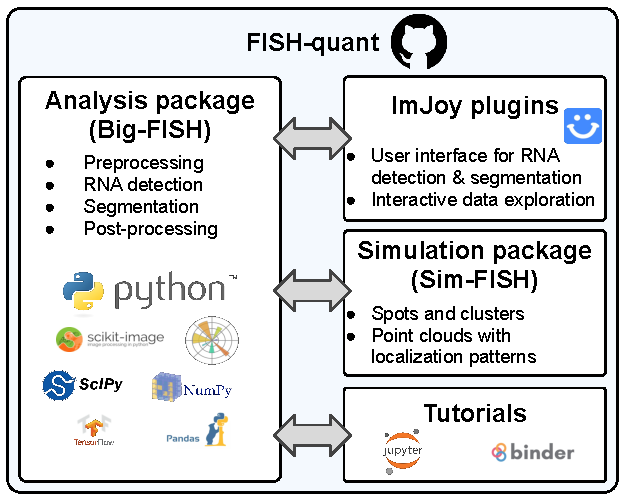
\includegraphics[width=0.8\textwidth]{figures/chapter1/schema_fishquant}
    \caption[Schematic view of FISH-quant]{Schematic view of FISH-quant.
	The software is hosted on GitHub and consists of several interconnected repositories.
	The Python core package \emph{bigfish} contains the entire analysis code, which is used by the ImJoy GUIs, the tutorial repository and a simulation package \emph{simfish}}
    \label{fig:fishquant}
\end{figure}

FISH-quant v2 is entirely open-source and hosted on GitHub under the FISH-quant organization\footnote{\url{https://github.com/fish-quant}}.
Using a GitHub organization allowed me to provide dedicated repositories with well defined and dedicated scope (see Figure~\ref{fig:fishquant}).
Further, it gives the flexibility for future extension where new projects can be integrated as new, independent repositories, without affecting and complexifying the already existing code.
The user can choose the adequate code for the analysis needs, without the overhead of installing unnecessary packages.
This GitHub organization is organized in several resources with dedicated repositories and documentation.

First, I implemented a Python package (\emph{bigfish}) providing the core code for performing scalable computation and analysis.
Second, I provide detailed interactive examples with test data for each analysis step that are available in Jupyter notebooks.
These examples can also be run directly on Binder~\cite{Jupyter2018Binder2}, a free and reproducible Jupyter notebook service, without local installation.
Third, a Python package (\emph{simfish}) allows the simulation of different subcellular \ac{RNA} localization patterns.
Fourth, ImJoy plugins~\cite{ouyang_imjoy_2019} provide a \ac{GUI} for the most commonly used workflows, and an interactive tutorial that can also run directly without local installation.
Lastly, a landing page\footnote{\url{https://fish-quant.github.io/}} centralizes implemented tools and directs new users to the most relevant resource for their analysis needs.

Dependencies for the Python packages are limited to standard Python scientific libraries: scientific computing (numpy~\cite{2020NumPy}, SciPy~\cite{2020SciPy}), data wrangling (pandas~\cite{mckinney_pandas_2010}), image analysis (scikit-image~\cite{walt_scikit-image_2014}), visualization (matplotlib~\cite{hunter_matplotlib_2007}), parallel computing (joblib\footnote{\url{https://github.com/joblib/joblib}})and machine learning (scikit-learn~\cite{scikit-learn}, TensorFlow~\cite{tensorflow_2015}).
The GitHub repositories are using continuous integration providing increased robustness of the released code, through unitary testing, version control and automatically generated up-to-date documentation.
Finally, packages are hosted under a BSD 3-Clause License.

\subsection{Big-FISH}
\label{subsec:bigfish}

\subsubsection{\emph{pip install big-fish}}

We chose to implement the core analysis package \emph{bigfish} in Python.
Compared to MATLAB, Python allows the development of a free and fully open-source software.
It also provides access to established libraries for data and image analysis, in addition to the most popular deep learning frameworks.
Lastly, Python packages can be interfaced with other tools and frameworks, from data analysis to web design, to provide interactive tools for user interaction and data inspection.

As shown in Figure~\ref{fig:bigfish}, \emph{bigfish} includes several independent subpackages for the different steps in a \ac{smFISH} analysis workflow: preprocessing, detection, segmentation, and analysis.
I designed each subpackage with clearly defined input and output data formats, which are automatically checked.
Each of these packages can be used independently in a modular fashion.
Users can thus create a customized analysis workflow, starting from preprocessing of images to statistical interpretation of results.
These workflows can be implemented in Python and Bash scripts and run both on local and remote computational resources.
The modular design also permits the easy integration of external methods, for instance, a new segmentation method can be combined with this spot detection algorithm.

More specifically, the Python code used in \emph{bigfish} package is organized in 7 subpackages performing dedicated steps:
\begin{itemize}
	\setlength\itemsep{0.1em}
	\item \emph{bigfish.stack} - I/O operations and images preprocessing
	\item \emph{bigfish.detection} - \ac{mRNA} spot detection
	\item \emph{bigfish.segmentation} - nucleus and cell segmentation
	\item \emph{bigfish.multistack} - post-processing and analysis of results from different channels, such as the merging of \ac{RNA} detections and segmentation masks or colocalization analysis
	\item \emph{bigfish.classification} - localization feature computation
	\item \emph{bigfish.plot} - visual reports of the obtained results
	\item \emph{bigfish.deep\_learning} - deep learning algorithms and pretrained models for segmentation or point cloud analysis
\end{itemize}

In this chapter, I provide only an overview of these subpackages.
More details can be found in subsequent chapters where I discuss particular algorithms that I have designed or implemented, or both.
I would also like to refer interested readers to the package documentation\footnote{\url{https://big-fish.readthedocs.io/en/stable/}} or the GitHub repository\footnote{\url{https://github.com/fish-quant/big-fish}}.
Dedicated notebook tutorials are also available\footnote{\url{https://github.com/fish-quant/big-fish-examples}}.
They can be run directly in the browser with Binder~\cite{Jupyter2018Binder2} and provided sample data, and thus allows new users to immediately test the package.

\begin{figure}[]
    \centering
    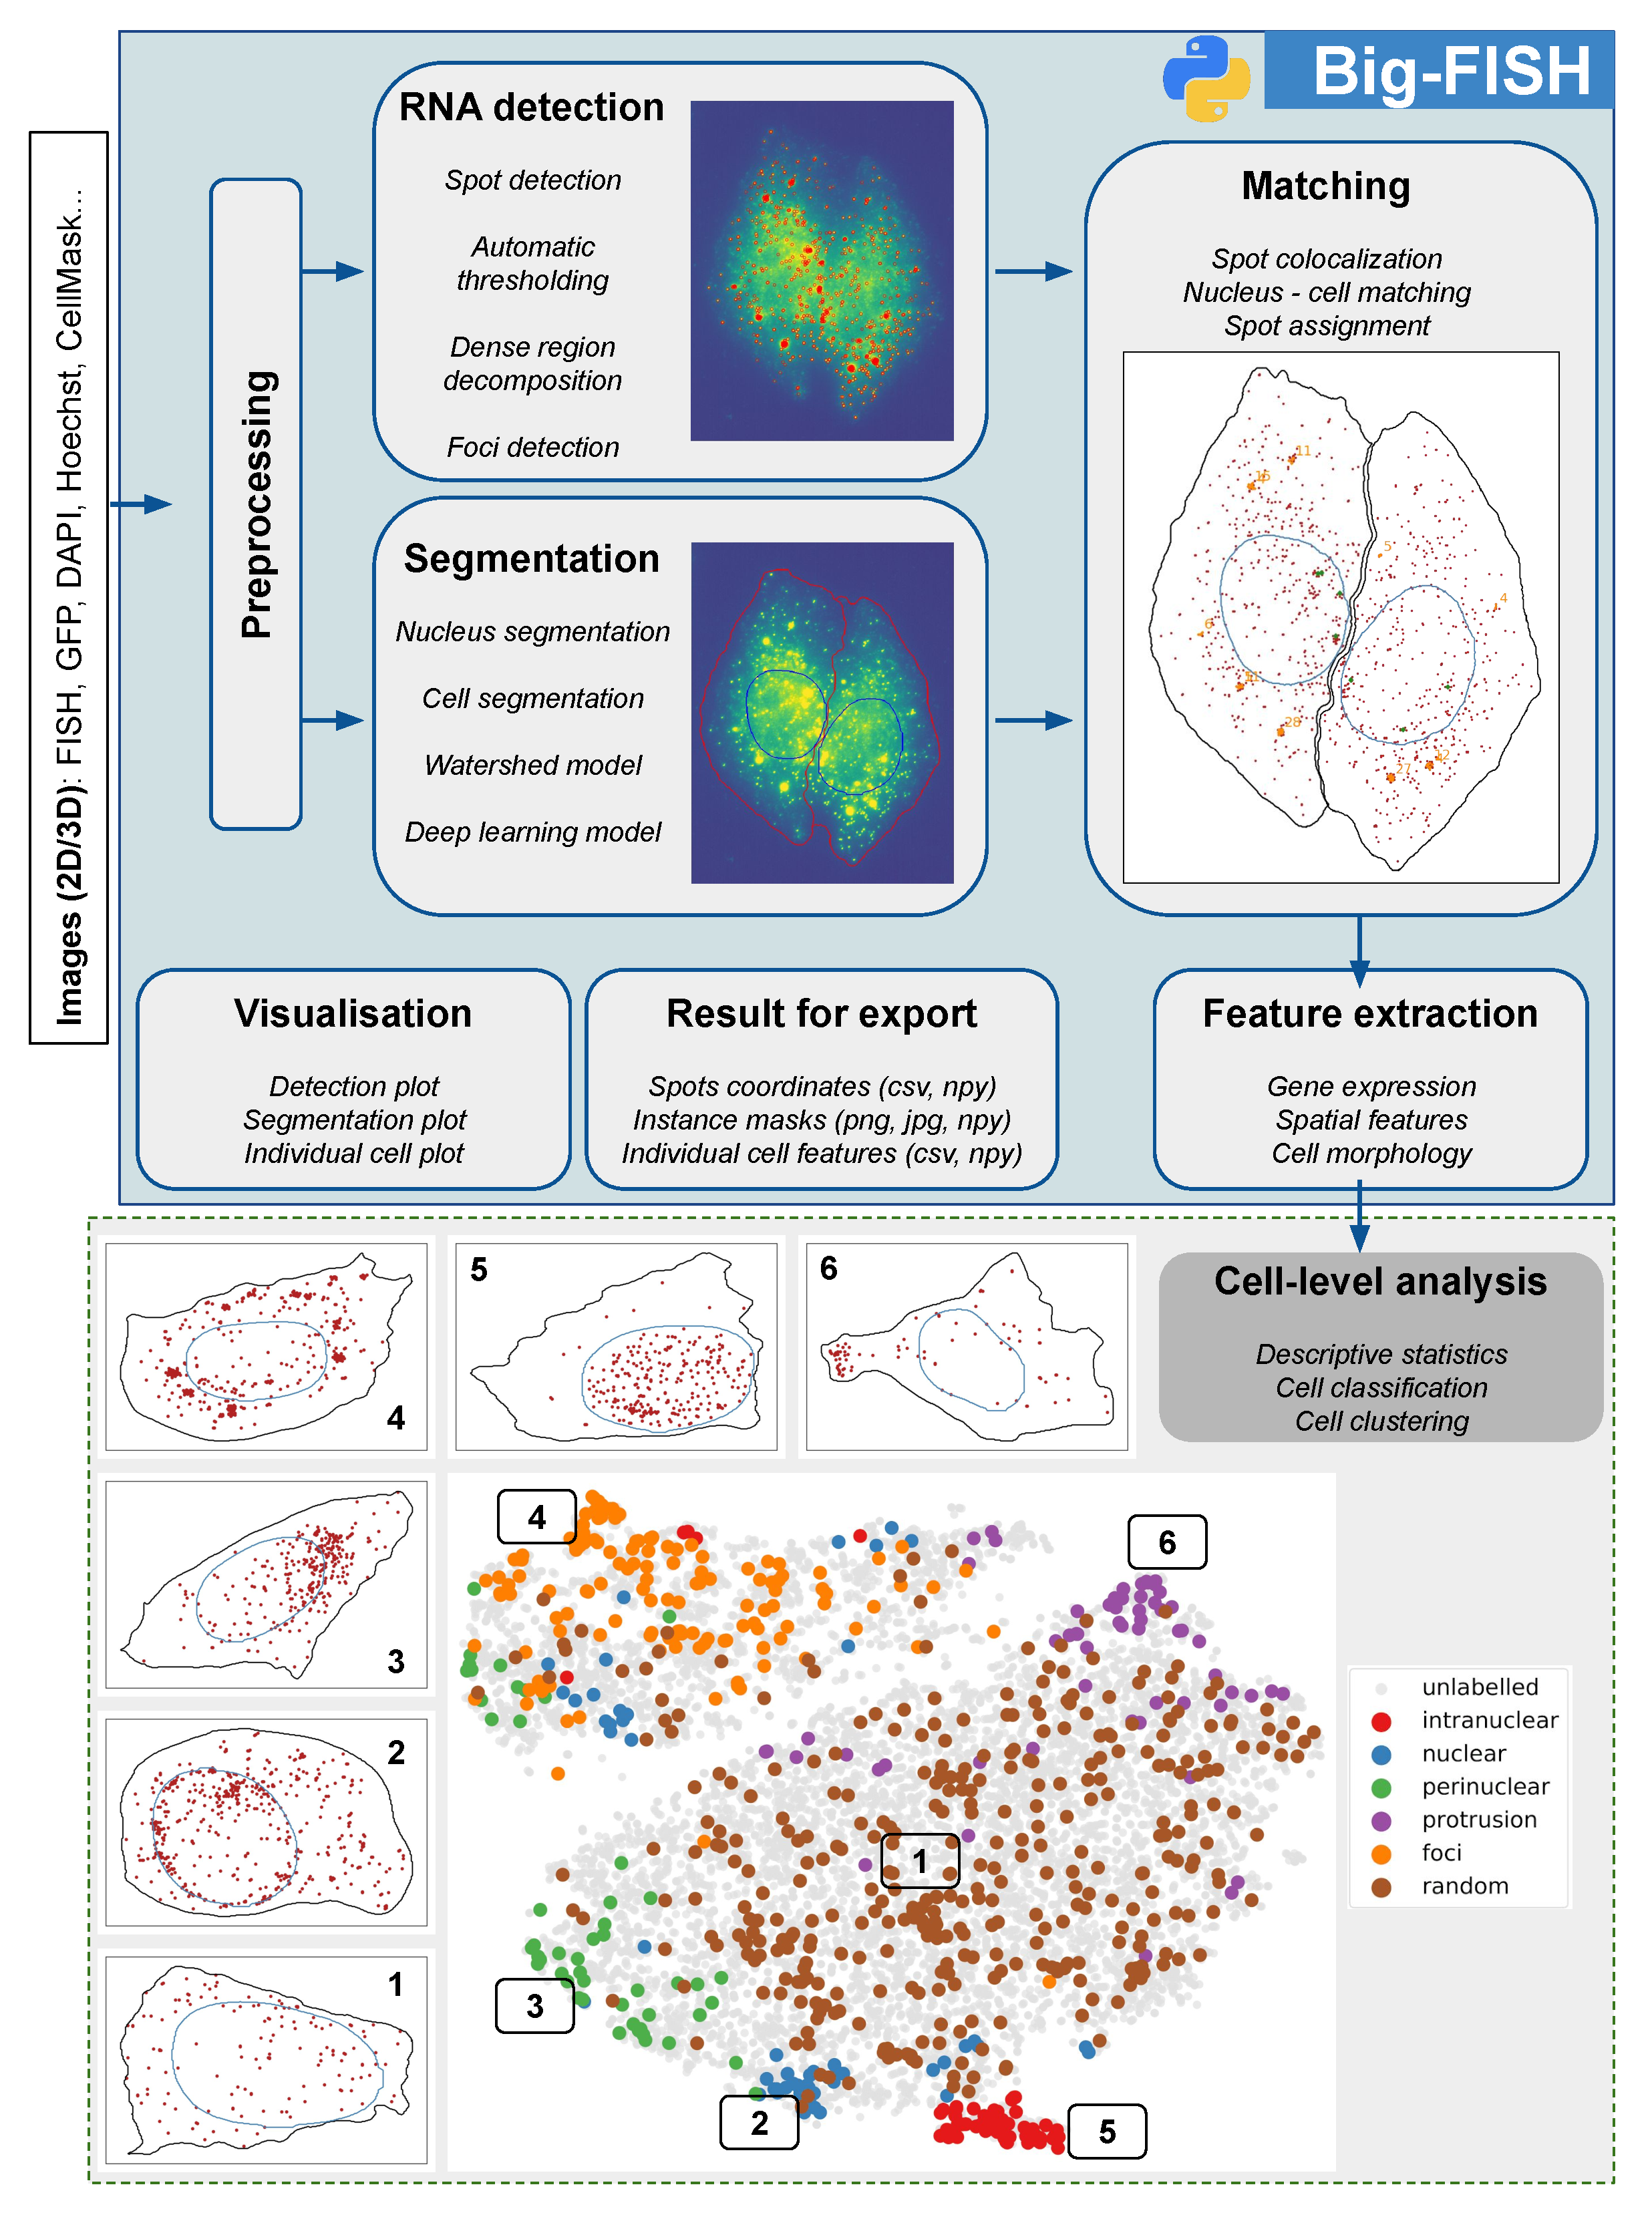
\includegraphics[width=0.95\textwidth]{figures/chapter1/schema_bigfish_full}
    \caption[Schematic view of \emph{bigfish}]{Schematic view of \emph{bigfish}.
	(\textit{Upper part}) Main modules illustrated with a typical analysis workflow.
	Shown are also the inputs and outputs that are created at the different steps.
	(\textit{Lower part}) Not directly included in \emph{bigfish}.
	As a final result, each cell is described with a set of features reflecting RNA abundance and localization.
	These features can then be used to perform analysis on the cell population.
	Results from~\cite{CHOUAIB_2020} are illustrated as example (see chapter~\ref{ch:chapter5} for more details).
	The t-SNE plot projects 15 localization features for smFISH experiments against 27 different genes.
	Each dot is one cell.
	The color-coded dots are manual annotations of six different localization patterns.
	Images are examples of individual cells displaying a typical localization pattern of this region of the t-SNE plot}
    \label{fig:bigfish}
\end{figure}

\subsubsection{Building blocks for a full analysis pipeline}

The package \emph{bigfish} aims at addressing the main challenges in \ac{smFISH} analysis.

First, for image handling and preprocessing, I implemented a number of different utility functions to read, write, normalize, cast, filter, and project images.
Different image file formats are natively supported and both 2D and 3D images can be processed.
These methods are gathered in \textbf{bigfish.stack}.

Second, the detection subpackage (\textbf{bigfish.detection}) provides methods required to detect spots in 2D or 3D images.
An important aspect of my implementation is its ability to detect spots without setting any pixel intensity threshold.
I propose a method to automatically infer this threshold from the image.
Such automatization overcomes human intervention and allows scaling to large data sets, such that the subpackage can process thousands of images.
While initially designed to detect individual \ac{mRNA}s, this subpackage permits the detection of larger spot-like structures like P-bodies or centrosomes (see applications in chapter~\ref{ch:chapter5} for more details).
Furthermore, I provide a fitting method to localize spots with a subpixel accuracy, a colocalization algorithm and cluster detection.
Strong local accumulation of \ac{RNA}s can lead to an underdetection since such accumulations are counted as single \ac{RNA}s.
For such cases, I also provide tools to decompose these dense regions and estimate the right number of spots.
The chapter~\ref{ch:chapter2} gives a comprehensive description of the implemented detection methods.

Third, the segmentation subpackage (\textbf{bigfish.segmentation}) contains several algorithms and utility functions for segmentation and post-processing.
It provides a simple deep-learning-based approach to segment cells and nuclei, but also traditional methods such as thresholding or watershed.
Furthermore, different post-processing tools are available to refine and clean the segmentation result, such as boundary smoothing, removal of small objects or filling of small holes.
These algorithms are presented with more details in the chapter~\ref{ch:chapter3}.

Forth, detected \ac{RNA} point clouds need to be matched to their cellular or subcellular environment.
For this, the subpackage \textbf{bigfish.multistack} enables to combine detection and segmentation results, obtained from different input channels.
It permits the analysis of \ac{RNA} abundance and distribution at the single-cell level.
Detected spots can be assigned to a specific region of interest, for instance, a cell or a nucleus.
Using the same method, \ac{RNA} clusters can be assigned to a nucleus and thus be considered as transcription sites.
\ac{RNA} expression levels are computed within this subpackage, as this is usually the minimum information that is extracted from a spatial transcriptomics study.

Finally, the subpackage \textbf{bigfish.classification} computes features at the single cell level from the spot positions and the coordinates of cellular landmarks.
These features allow a statistical description of the cell population or can feed a classification model allowing for the discrimination of individual cells according to their RNA localization patterns.
More information about the cell matching step and the feature engineering are presented in chapter~\ref{ch:chapter4}.

In \emph{bigfish}, I also provide a subpackage (\textbf{bigfish.plot}) to visualize the results of each intermediate step in the analysis workflow and thus provide valuable visual quality control.
A last subpackage (\textbf{bigfish.deep\_learning}) gathers the utility functions and model architectures to run deep learning solutions.
The use of such techniques implies more complex dependencies in the back-end like TensorFlow~\cite{tensorflow_2015}.
By isolating pieces of code related to deep learning, I make the import of these frameworks optional for the user.
Indeed, the majority of the methods provided by \emph{bigfish} does not require artificial neural networks.

\subsection{Sim-FISH}
\label{subsec:simfish}

The Python package \emph{simfish} is dedicated to the simulation of \ac{FISH} images.
These simulations come in two flavors: simulation of \ac{smFISH} image simulation and simulation of point cloud coordinates with a specific localization patterns.

Spots or clusters of spots with various intensities and shapes can be simulated, in 2D or 3D, optionally with subpixel accuracy.
Different parameters, such as the number of spots, the size of the clusters and even the background noise level or randomness in the image can be controlled by the user.
These simulated images can be used to validate spot or cluster detection methods, for instance to evaluate the impact of varying noise levels.
I refer to the chapter~\ref{ch:chapter2} for the details about the generation of these images.

The simulated point clouds are used to build a large dataset with different \ac{RNA} localization patterns.
They can be used for benchmarking and ultimately for the training of neural networks for classification of localization patterns.
The output of the simulation is not an image, but a list of 3D \ac{RNA} coordinates as well as the 2D cell and nuclear boundaries.
The localization pattern can be chosen among 9 predefined patterns, and the strength of the pattern (and thus the difficulty of recognizing the pattern) can be controlled by one parameter.
Chapter~\ref{ch:chapter4} provides a thorough description of the simulations.

More generally, such simulations can be helpful to validate, calibrate or pre-train algorithms.
This is particularly true when we deal with experimental data difficult to generate or annotate.
Lastly, online information about the simulation package are available in the documentation\footnote{\url{https://sim-fish.readthedocs.io/en/stable/}} or in the GitHub repository\footnote{\url{https://github.com/fish-quant/sim-fish}}.

\subsection{ImJoy}
\label{subsec:imjoy}

\begin{figure}[]
    \centering
    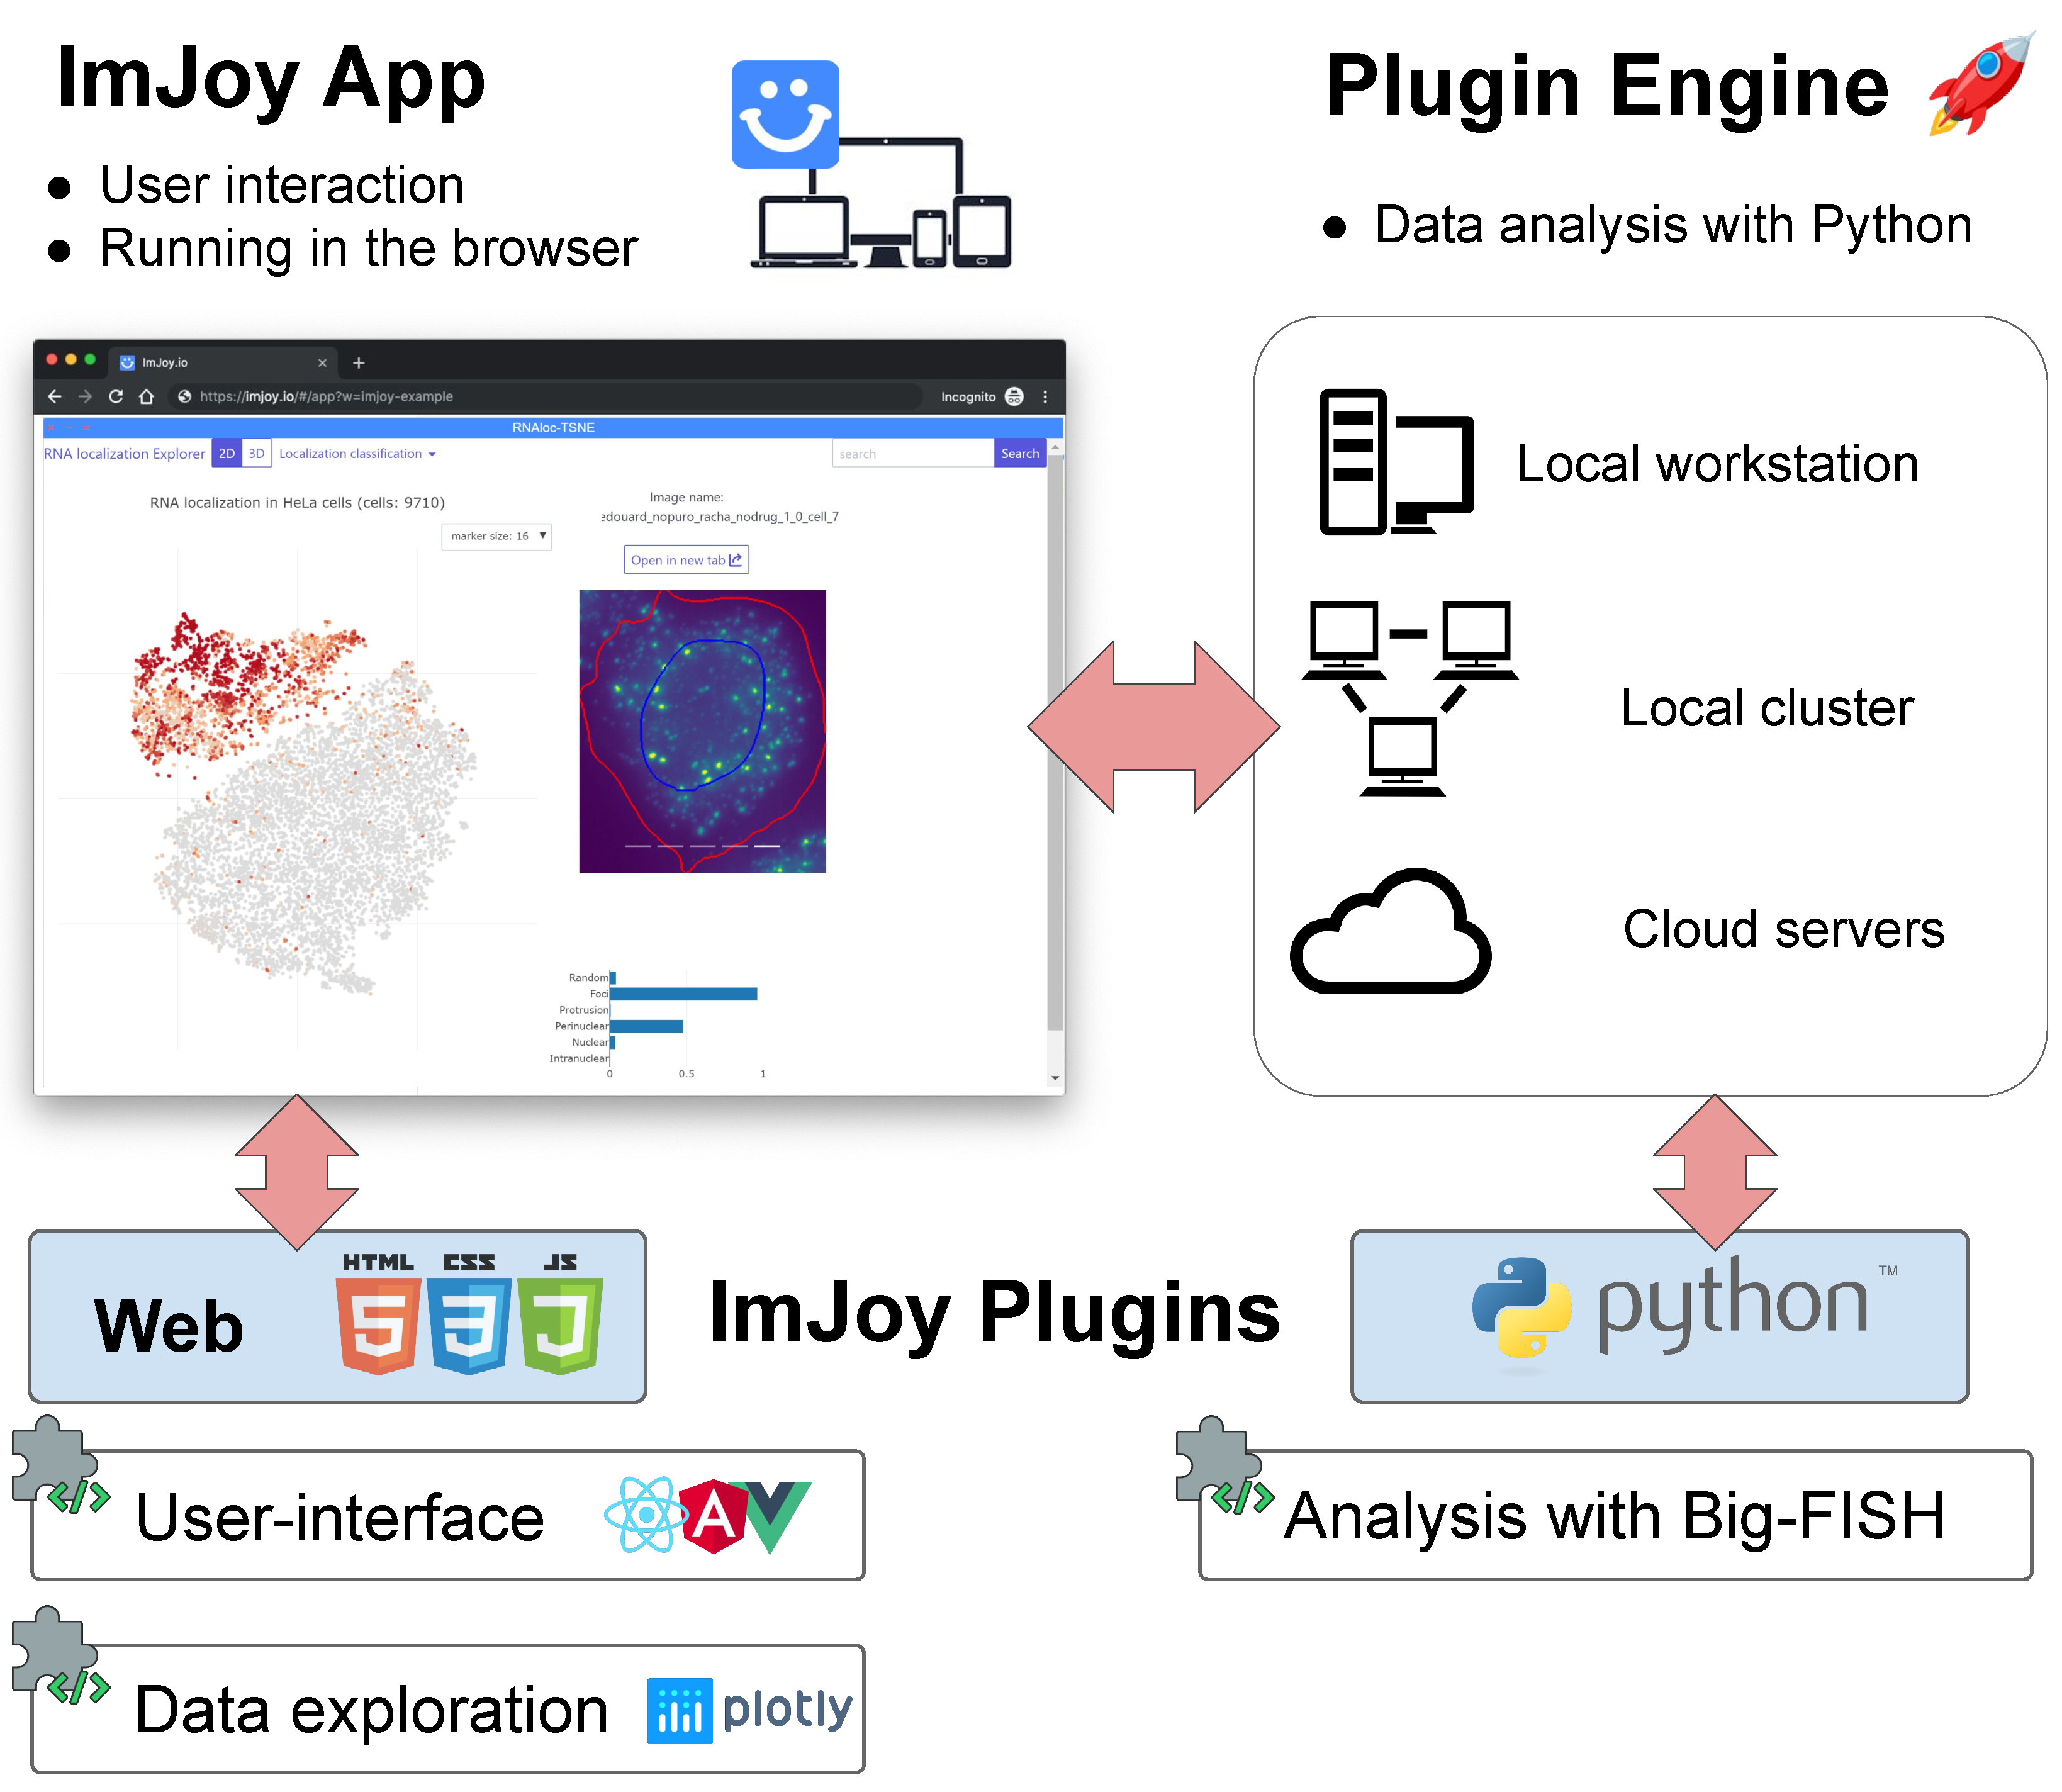
\includegraphics[width=0.8\textwidth]{figures/chapter1/schema_imjoy}
    \caption[Schematic view of ImJoy]{Schematic view of ImJoy.
	(\textit{Top}) ImJoy's core is a Progressive Web App whose functionalities are provided by plugins run directly in the browser or on a plugin engine (local or remote).
	Plugin engines support the scientific Python ecosystem and dependency management is handled with Conda.
	(\textit{Bottom}) Browser plugins are implemented with HTML, CSS or JavaScript.
	They allow user interaction, data visualization and computation in the browser.
	Heavier computations can be run from a Python plugin engine before being displayed in the web app}
    \label{fig:imjoy}
\end{figure}

The \emph{bigfish} package provides flexibility and scalability since its components can be adapted to the specific analysis needs of a given project.
However, it requires at least a minimum knowledge of Python to establish a complete workflow by using the provided tutorials.
We thus implemented several plugins with a \ac{GUI} for ImJoy ~\cite{ouyang_imjoy_2019}.
A general organization of ImJoy is illustrated in Figure~\ref{fig:imjoy}.
It provides simpler access for users with no computational background and no programming skills.
These plugins provide the most commonly used analysis workflow, as determined from the usage of the Matlab version of FISH-quant~\cite{mueller_fish-quant_2013}, and will thus be suited for a large number of use cases.
It mostly includes segmentation and detection tools.

First, we implemented a plugin to perform segmentation on top of CellPose model~\cite{stringer_cellpose_2021}.
Thanks to the modular design, this model can be easily exchanged if more performant methods are available in the future.
A documentation is available online to launch and run the plugin\footnote{\url{https://fq-segmentation.readthedocs.io/en/latest/}}.

We also implemented a detection plugin based on \emph{bigfish} modules.
Both isolated and clustered \ac{RNA} can be detected and detection results can be inspected with the Kaibu image viewer plugin in ImJoy.
While \emph{bigfish} is developed to be scalable without the need to fine tune parameters, different detection settings can be interactively investigated through the \ac{GUI}.
Batch processing of entire folders is also possible.
Lastly, detection results can be assigned to segmented cells and nuclei if segmentation masks are available.
An online documentation is available for this plugin\footnote{\url{https://fq-imjoy.readthedocs.io/en/latest/}}, and also an interactive demo\footnote{\url{https://fish-quant.github.io/fq-interactive-docs/\#/fq-imjoy}}.
This demo can be run directly in the browser without any local installation.

Using ImJoy provides several advantages compared to a stand-alone \ac{GUI}.
Due to its distributed design that separates \ac{GUI} from computation plugins, it natively supports user-friendly remote computing which allows access to massive data storage and powerful computation resources including GPUs.
ImJoy is a Progressive Web App where the user interface plugin is implemented with front-end languages like HTML, CSS or JavaScript.
It then transparently calls the \emph{bigfish} methods running on a Python plugin engine (for example a Jupyter notebook server) to perform the actual \ac{smFISH} analysis task.
While this plugin can run on a local workstation, it can be executed on a computational cluster or even in the cloud or seamlessly switching between them.
For example in our demo version, the engine is running on Binder~\cite{Jupyter2018Binder2}.
Once the plugin engine is installed on the remote resource, the end-user can connect with ImJoy and will be confronted with the same interface (the browser plugin), independently of where the analysis is actually performed.
Interestingly, this front-end interface can also be opened with mobile devices.
ImJoy plugins implemented in JavaScript not only provide modern and reactive user interfaces, but also profit from the extensive JavaScript resources in terms of data visualization and interactivity.
Such interactivity is becoming increasingly important, especially when large and complex data sets are analyzed where static plots are too limited.
As a case example, we provide an interactive t-SNE plot\footnote{\url{https://fish-quant.github.io/fq-interactive-docs/\#/rnaloc-tsne}} for the data analyzed in~\cite{CHOUAIB_2020} and detailed in chapter~\ref{ch:chapter5}.
This plugin can be run without local installation and enables the user to explore and interact with these complex data.

\section{Conclusion}
\label{sec:conclusion}

In this chapter I present the second version of FISH-quant, a user-friendly Python based framework for the complete analysis of \ac{smFISH} images.
It is built around \emph{bigfish}, a core-analysis package, implemented following rigorous software development guidelines, with detailed interactive documentation and tutorials.
This package consists of several interchangeable modules whose organization matches key steps in \ac{smFISH} image analysis: preprocessing, \ac{RNA} detection, cell segmentation and analysis.
Its modularity permits the creation of flexible workflows ranging from the analysis of small data sets with the help of a \ac{GUI} to custom-tailored investigation of large-scale screens requiring computational clusters.
Indeed, I also provide user interfaces in ImJoy accessible to biologists without programming skills, which can be used locally or scaled to larger remote computational resources, and displayed in the browser.
A last package, \emph{simfish}, allows the simulation of \ac{smFISH} images with non random \ac{RNA} localization patterns.
These simulations can be used to develop and evaluate analysis pipelines.
Lastly, the use of Python scientific ecosystem, as well as strict version control and minimal dependencies, facilitate installation, maintenance and integration with other analysis or visualization frameworks.
All dependencies, as well as FISH-quant v2, are open-source, thus can be used free of charge.

In the chapters~\ref{ch:chapter2},~\ref{ch:chapter3} and~\ref{ch:chapter4}, I detail the different functions available in FISH-quant.
Throughout the manuscripts, I thus include several snippets with the few lines of code related to the described methods.
